% Chapter 3

\chapter{Teoria de Antenas} % Main chapter title
\label{chap:Chapter3} % For referencing the chapter elsewhere, use \ref{chap:Chapter3} 

%----------------------------------------------------------------------------------------
\section{Teoria Básica de Antenas}
Uma antena é definida como "um dispositivo geralmente metálico (com haste ou fio) para irradiar ou receber ondas de rádio" \parencite{Balanis2016}, ou seja, uma antena, é o dispositivo que permite a transição entre o meio que a rodeia e o equipamento, que se pode observar na Figura \ref{fig:antena transicao}. 
Este dispositivo é um transdutor que converte energia elétrica em ondas eletromagnéticas ou vice versa, sendo que é uma antena de transmissão, se converter um sinal elétrico num sinal eletromagnético e é uma antena de receção, se converter um sinal eletromagnético em sinal elétrico. 

\begin{figure}[h]
\centering
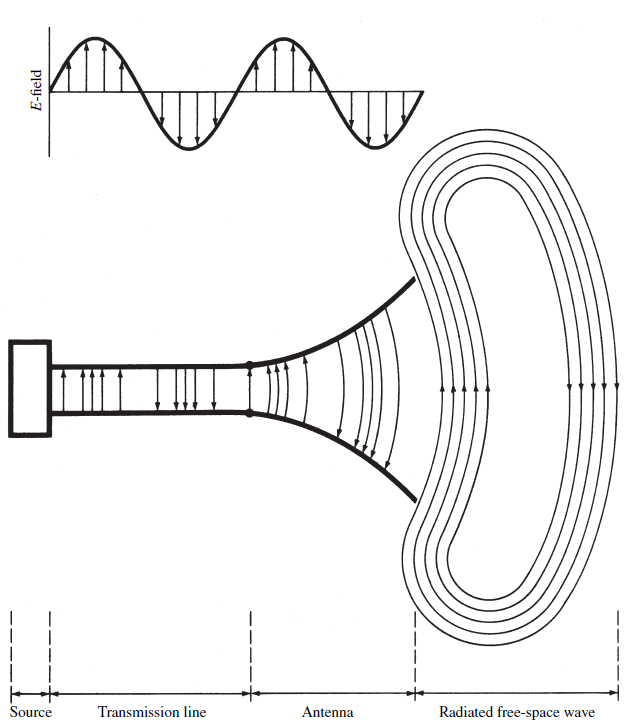
\includegraphics[scale=0.6]{chapters/ch3/assets/Antenna_transicao}
\decoRule
\caption[Antena como meio de transição]{Antena como um meio de transição (Figura 1.1 - \cite{Balanis2016})}
\label{fig:antena transicao}
\end{figure}

\subsection{Tipos de Antenas}
Neste subcapítulo irá ser introduzido de uma forma breve, os vário tipos de antenas, a sua utilização e vantagens entre estes. 

\subsection*{Antenas de Fio}
Estas antenas são umas das mais antigas, que apresentam uma configuração mais simples, como se pode observar na Figura \ref{fig:wire antenna}, sendo apenas constituídas por um fio que pode variar na sua dimensão e na sua forma e ainda podem ser utilizadas nas mais variadas aplicações. Podem tomar uma forma aleatória, desde um fio direito (dipolo) até um fio com as mais diversas formas. \par 
As antenas de fio podem ser encontradas nos mais variados locais, desde aeronaves, carros ou navios a edifícios.

\begin{figure}[h]
\centering
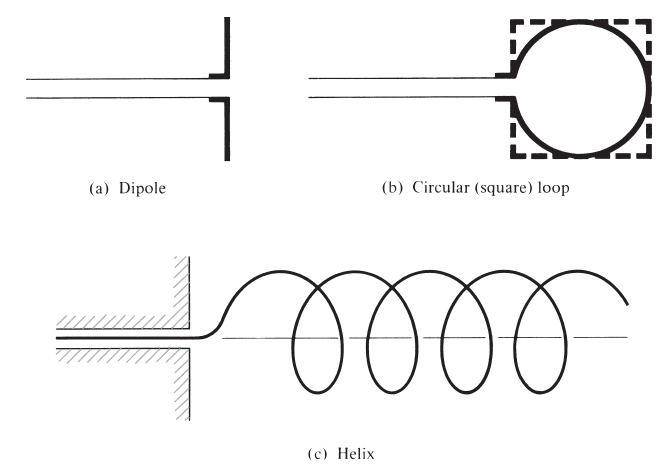
\includegraphics[scale=0.6]{chapters/ch3/assets/wire_antenna}
\decoRule
\caption[Antena de Fio]{Exemplos de vários tipos de antenas de fio (Figura 1.3 - \cite{Balanis2016})}
\label{fig:wire antenna}
\end{figure}

\subsection*{Antenas de Abertura}
Os campos no fim de um guia de ondas aberto não são uniformes devido a esta mesma abertura, assim, para este caso, assume-se que os campos são iguais a como se o guia de ondas continuasse fechado. As antenas de abertura entram quando se pretende aumentar a diretividade à saída do guia, abrindo as extremidades do mesmo de forma a dar uma forma como se observa na Figura \ref{fig:aperture antenna2}. Este tipo de antenas, em especifico as antenas de abertura piramidais, são utilizadas para alimentar ou calibrar grandes antenas de prato.\par
Assim sendo, as antenas de abertura são utilizadas para frequências mais elevadas, especificamente em frequências de micro-ondas e podem ser aplicadas nas mais variadas formas geométricas, como retangulares, elípticas, circulares, piramidais, entre outras.

\begin{figure}[h]
\centering
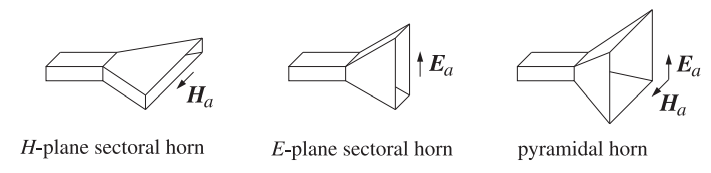
\includegraphics[scale=0.6]{chapters/ch3/assets/aperture_antenna2}
\decoRule
\caption[Antena de Abertura]{Antenas de abertura no plano H, E e piramidal}
\label{fig:aperture antenna2}
\end{figure}


\subsection*{Antenas de \textit{Microstrip}}
Uma antena \textit{microstrip}, conhecida como antena impressa, é um tipo de antena que está inserida numa placa de circuito impresso e funciona como uma antena interna.\par
Hoje em dia são utilizadas em aplicações comerciais, tendo como as suas maiores vantagens o facto de serem baratas e simples de manufaturar e apresentarem um tamanho reduzido. Este tipo de antenas são aplicadas em frequências \gls{UHF}.\par 
A sua construção consiste num \textit{patch} metálico sobre um substrato. Este \textit{patch} pode apresentar as mais variadas formas como representado na Figura \ref{fig:microstrip}, sendo as retangulares e circulares as mais comuns. Têm ainda as vantagens de serem impressas em superfícies com as mais variadas formas, sendo robustas e versáteis nos parâmetros da sua frequência de ressonância, polarização e impedância (\cite{Balanis2016}).

\begin{figure}[h]
\centering
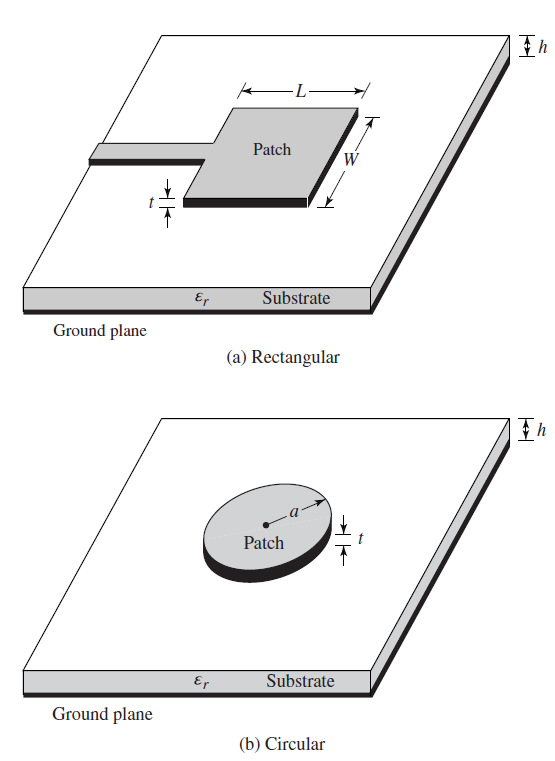
\includegraphics[scale=0.6]{chapters/ch3/assets/microstrip}
\decoRule
\caption[Antena \textit{Microstrip}]{Exemplos de duas configurações de \textit{patches} diferentes (Figura 1.5 - \cite{Balanis2016})}
\label{fig:microstrip}
\end{figure}

\subsection*{Antenas de Matrizes}
As antenas de matrizes surgem nas aplicações em que é necessário mais que um elemento. Consegue-se assim agrupar vários elementos de forma a obter as características pretendidas. Algumas alterações às caraterísticas que se conseguem com este tipo de antenas antenas são o aumento de ganho, alterar o diagrama de radiação, determinar a direção de chegada de um sinal ou maximizar o \gls{SINR}\footnote{\gls{SINR} é um indicador de qualidade de transmissão ajustado a comunicações móveis devido à interferência de outros utilizadores ser mais significativa \parencite{Jeske2004}.}.

\subsection*{Antenas de Lente}
Este tipo de antenas utiliza as propriedades de convergência e divergência das lentes para a receção ou transmissão de sinal. O tamanho da lente a ser utilizada depende da frequência - quanto maior for a frequência, menor a lente. Dito isto, é mais favorável usar este tipo de antenas em frequências mais altas, visto que a lente será menor. As suas aplicações são semelhantes às das refletoras parabólicas, especificamente quando usadas em frequências mais altas e que necessitem de mais largura de banda.

\subsection*{Antenas Refletoras}
As antenas refletoras existem desde o final do século XIX, no entanto começaram a ser aplicadas em radares na Segunda Guerra Mundial e a partir do final do século XX em comunicações espaciais. Estas aplicações devem-se à sua capacidade de transmissões a grandes distâncias. Podem-se apresentar nas mais diversas formas, como plano refletor, refletor curvilíneo, entre outros.\par 
O seu modo de funcionamento baseia-se na convergência da energia numa direção como demonstrado na Figura \ref{fig:reflector}, o que leva, para além de um grande alcance, a uma grande diretividade.

\begin{figure}[h]
\centering
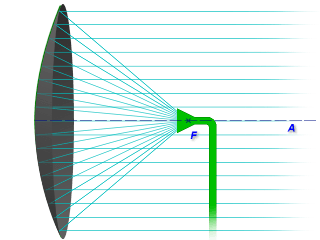
\includegraphics[scale=0.6]{chapters/ch3/assets/reflector}
\decoRule
\caption[Antena Refletora]{Funcionamento de uma Antena Refletora}
\label{fig:reflector}
\end{figure}

\subsection{Parâmetros Fundamentais}
Neste subcapítulo vão ser discutidos os parâmetros fundamentais para o funcionamento de uma antena e a sua \textit{performance}. Grande parte dos parâmetros estão definidos no IEEE 1983 Standard Definitions for Antennas and Propagation.

\subsection*{Diagrama de Radiação}
Um diagrama de radiação é a função ou representação gráfica que descreve as propriedades espaciais de radiação de uma antena. É de extrema importância conhecer este padrão de radiação de uma antena e poder controla-lo, visto que a distribuição de energia eletromagnética, se for mal dimensionada, pode comprometer o projeto. \par 

A manipulação do diagrama de radiação de uma antena é dependente do objetivo da mesma. Podemos ter como finalidade um diagrama de radiação que seja direcional (Figura \ref{fig:direcional}), como numa ligação ponto a ponto, ou podemos como finalidade, um diagrama de radiação omnidirecional (Figura \ref{fig:omnidirecional}), ou seja, que radia, idealmente, com igual intensidade para todas as direções.\par

Para este efeito são utilizadas coordenadas esféricas ($r$, $\varphi$ e $\theta$), sendo que a antena se encontra na origem do referencial. A propriedade mais relevante nos diagramas de radiação é a distribuição espacial, em duas ou três dimensões, da energia radiada em função da posição do observador de acordo com um azimute ($\theta$ constante).\par 

\begin{figure}[h]
\centering
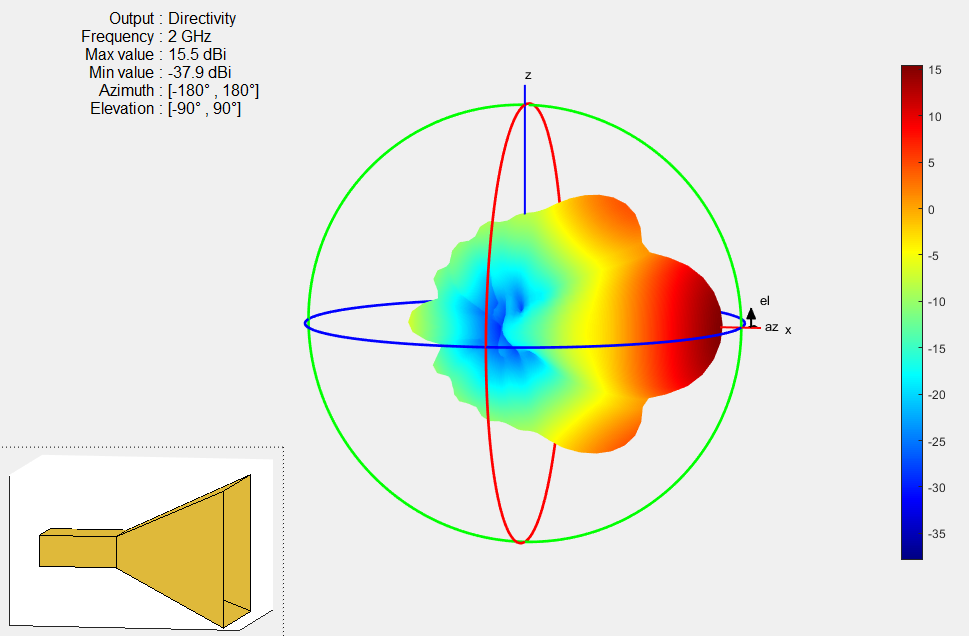
\includegraphics[scale=0.6]{chapters/ch3/assets/matlab_ad1}
\decoRule
\caption[Diagrama de radiação direcional]{Diagrama de radiação direcional - Corneta de guia de ondas dimensionada para 1GHz (MATLAB Antenna Designer Toolkit)}
\label{fig:direcional}
\end{figure}

\begin{figure}[h]
\centering
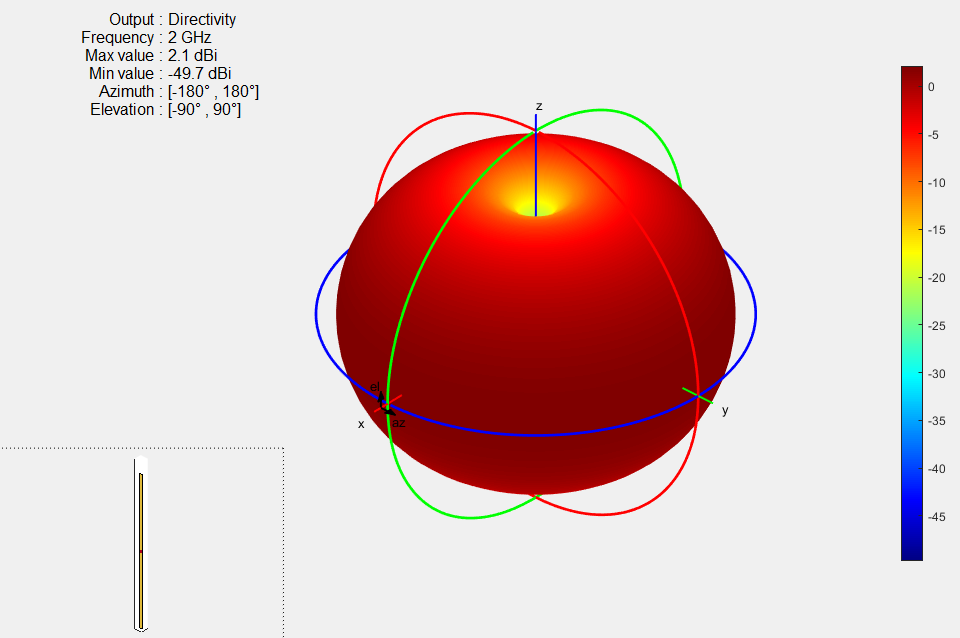
\includegraphics[scale=0.6]{chapters/ch3/assets/matlab_ad2}
\decoRule
\caption[Diagrama de radiação omnidirecional]{Diagrama de radiação omnidirecional - Dipolo dimensionado para 2GHz (MATLAB Antenna Designer Toolkit)}
\label{fig:omnidirecional}
\end{figure}

Os lóbulos são um dos parâmetros fundamentais de um diagrama de radiação, que representam a energia radiada numa direção relativamente ao transmissor e podem ser classificados em lóbulos principais, secundários, laterais e posteriores (Figura \ref{fig:elem_carat_dg}). O lóbulo principal é o lóbulo que contém a direção da radiação máxima, que no caso da Figura \ref{fig:elem_carat_dg}, está definido no sentido do eixo dos zz. Os lóbulos secundários são todos os lóbulos expecto o principal. Os lóbulos laterais são todos os que radiam energia para qualquer direção que não seja a pretendida. Os lóbulos posteriores contêm a energia que é radiada num ângulo de 180$^{\circ}$ em relação à direção do feixe da antena. \par 

A largura de feixe a meia potência (\gls{HPBW}) e a largura de feixe ao primeiro nulo (\gls{FNBW}) estão relacionadas com a capacidade de resolução da antena, ou seja, a sua capacidade de distinguir dois alvos. O critério para distinguir dois alvos é que a \gls{HPBW} seja aproximadamente \gls{FNBW}/2, isto é, se dois alvos estiverem separadas por distâncias angulares iguais ou superiores a \gls{HPBW}$\approx$\gls{FNBW}/2 de uma antena, esta consegue distingui-los \parencite{Kraus1988}. Os fatores que afetam a largura de feixe são o comprimento de onda ($\lambda$), a forma do diagrama de radiação e as dimensões da antena. \par 

\begin{figure}[h]
\centering
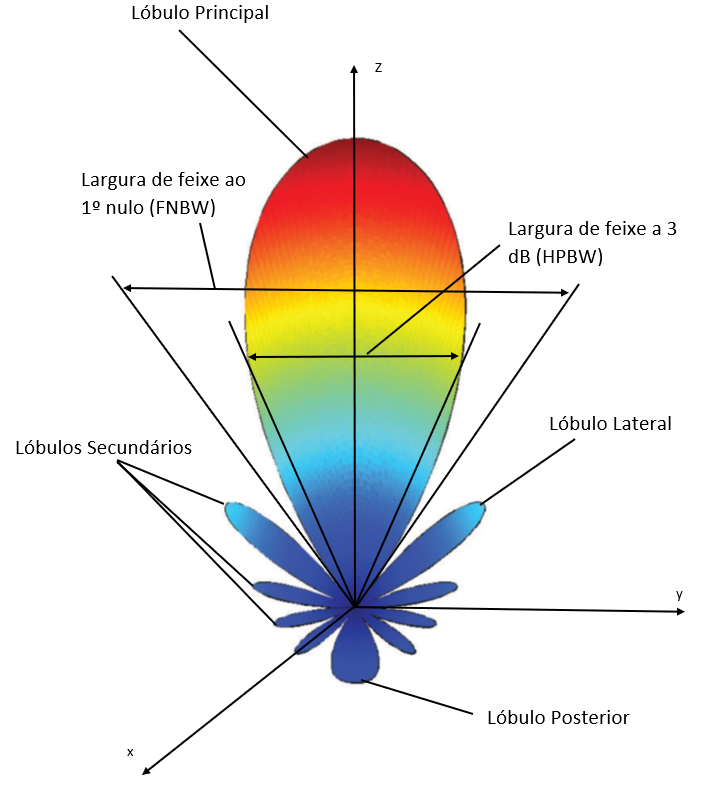
\includegraphics[scale=0.6]{chapters/ch3/assets/elem_carat_dg}
\decoRule
\caption[Elementos caraterísticos do diagrama de radiação]{Elementos caraterísticos do diagrama de radiação}
\label{fig:elem_carat_dg}
\end{figure}

Os diagramas de radiação podem ser classificados quanto à diretividade em que as antenas radiam. Um radiador isotrópico é definido com uma antena hipotética e sem perdas que radia igualmente em todas as direções e é normalmente tomado como referência para exprimir a diretividade de antenas. o radiador direcional é caracterizado por radiar ondas eletromagnéticas em determinadas direções e o radiador omnidirecional radia energia de igual forma em todas as direções \parencite{Balanis2016}.

\subsubsection*{Planos Principais}
Para antenas com polarização linear, discutido com mais detalhe no subcapítulo Polarização, consideram-se os seguintes planos:
\begin{itemize}
\item Plano E: Definido pelo plano que contém o vetor do campo elétrico e a direção da máxima radiação;
\item Plano H: Definido pelo plano que contém o vetor do campo magnético e a direção da máxima radiação.
\end{itemize}
Os eixos do sistemas de coordenadas são escolhidos por forma a que pelo menos um dos planos referido coincidas com os planos do referencial, no entanto, há casos em que pode ser mais favorável escolher outro sistema de coordenadas.


\begin{figure}[h]
\centering
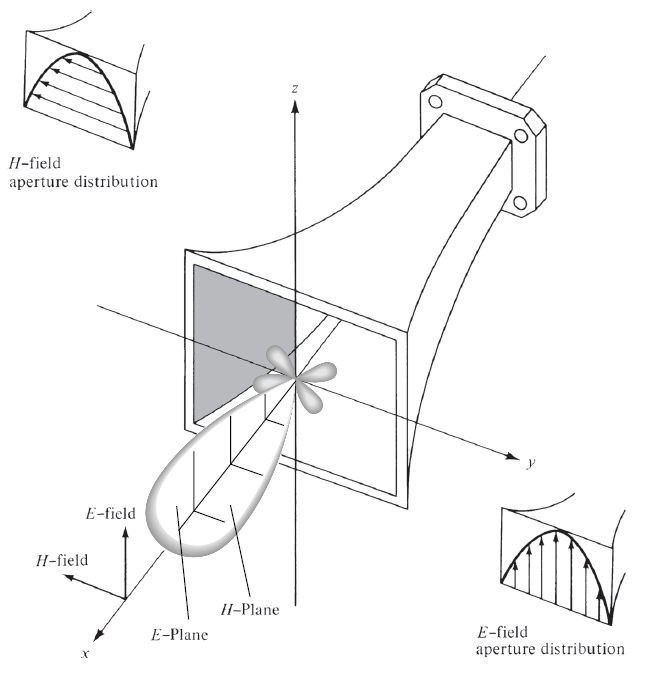
\includegraphics[scale=0.6]{chapters/ch3/assets/campoEH_piramidal}
\decoRule
\caption[Campos E e H de um diagrama de radiação de uma antena]{Campos E e H de um diagrama de radiação de uma antena}
\label{fig:campoEH_piramidal}
\end{figure}

\subsubsection*{Regiões de Campo}
De forma a identificar a estrutura do espaço circundante da antena, este é dividido em três regiões \parencite{Kraus1988}:
\begin{itemize}
\item Região reativa do campo próximo: Definida com a porção do espaço imediatamente em redor da antena, onde predomina o campo reativo;
\item Região do campo próximo (\textit{Região de Fresnel}): Definida como a região da antena entre a região reativa do campo próximo e a região de \textit{Fraunhofer} onde predomina o campo radiado e a sua orientação espacial depende da distância à antena;
\item Região do campo distante (\textit{Região de Fraunhofer}): Caraterizada pela região onde a distribuição angular do campo é maioritariamente independente da distância à antena.
\end{itemize}

Tipicamente, a forma diagrama de radiação é alterado consoante as regiões em que se encontra. Segundo a Figura \ref{fig:alt_tipicas_regioes} presente no artigo \cite{Y.RahmatL.WilliamsR.Yoccarino1995}, o diagrama é mais disperso e uniforme na região reativa do campo próximo. À medida em que a distância à antena aumenta, e que se entra nas regiões de \textit{Fresnel} e \textit{Fraunhofer} a forma do diagrama evidencia mais os seus lóbulos e fica mais regular. A separação entre as regiões reativa do campo próximo e região de \textit{Fresnel} e entre a região de \textit{Fresnel} e região de \textit{Fraunhofer} são definidas pelas expressões \ref{3.1} e \ref{3.2} respetivamente \parencite{Y.RahmatL.WilliamsR.Yoccarino1995}.

\begin{equation} \label{3.1}
R=\dfrac{2D^{2}}{\lambda}
\end{equation}

\begin{equation} \label{3.2}
R=0.62\sqrt{\dfrac{D^{3}}{\lambda}}
\end{equation}

\begin{figure}[h]
\centering
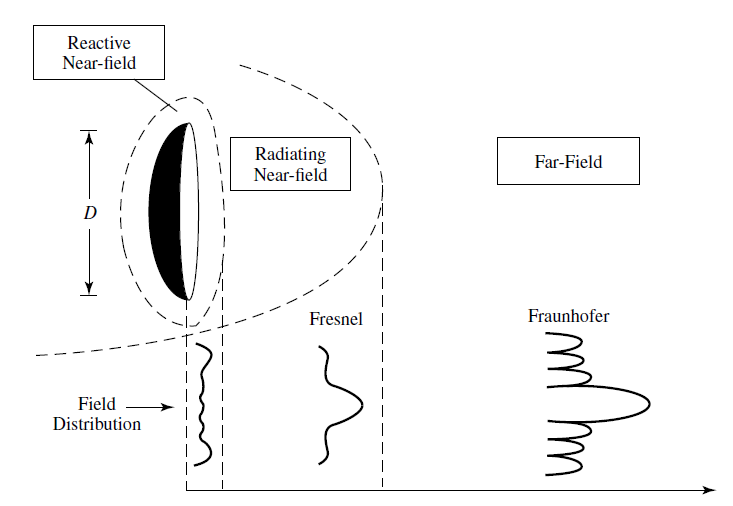
\includegraphics[scale=0.6]{chapters/ch3/assets/alt_tipicas_regioes}
\decoRule
\caption[Alterações típicas da forma do diagrama de radiação]{Alterações típicas do diagrama de radiação desde a reagião reativa do campo próximo à \textit{Região de Fraunhofer}. \parencite{Y.RahmatL.WilliamsR.Yoccarino1995}}
\label{fig:alt_tipicas_regioes}
\end{figure}


\subsection*{Densidade de Potência}

As ondas eletromagnéticas resultam da combinação de um campo magnético e de um campo elétrico que se propaga no espaço. A forma de representar a densidade direcional da quantidade de energia transferida de uma onda eletromagnética é através do vetor de \textit{Poynting}, o qual é definido, contabilizando variações temporais sinusoidais, na equação \ref{3.3}, expressa em \si{\watt\per\meter\squared}.

\begin{equation} \label{3.3}
W_{av}(x,y,z)=\dfrac{1}{2}Re[E\times H^{*}]
\end{equation}

Sendo que o vetor de \textit{Poynting} é uma densidade de potência, ao integrar a componente normal do mesmo ao longo da superfície S, obtém-se na equação \ref{3.4} a potência média radiada pela antena $P_{rad}$.

\begin{equation} \label{3.4}
P_{rad}=P_{av}=\oint_S W_{rad}\cdot ds 
=\dfrac{1}{2} \oint_S Re[E\times H^{*}]\cdot ds
\end{equation}

 
\subsection*{Intensidade de Radiação}


\subsection*{Diretividade}


\subsection*{Ganho}


\subsection*{Largura de Banda}


\subsection*{Polarização}


\subsection*{Impedância de Entrada}


\subsection*{Eficiência}
\subsubsection*{Eficiência da Antena}


\subsection*{Máxima Diretividade e Máxima Área Efetiva}



\subsection*{Equação de Friis e Equação Radar}



\subsection*{\textit{Radar Cross Section}}



\subsection*{Temperatura da Antena}


\subsection*{Síntese}




\section{Simulação de uma Antena}


\subsection{Para Sinais DVB-T}

